% !TEX program = lualatex
% !TEX options = -synctex=1 -interaction=nonstopmode -file-line-error -shell-escape -halt-on-error %DOC%
% !TEX encoding = UTF-8 Unicode

\documentclass[twoside, a4paper]{extreport}
\usepackage{scrextend}
\changefontsizes{16pt} % ustawia 16pt jako bazę dla całego dokumentu
% -----------------------------------------------------------------------------------
% ------------------------- USTAWIENIA STRONY--------------------------
% -----------------------------------------------------------------------------------
\usepackage{geometry}
\geometry{
	left=10mm,
	right=10mm,
	top=15mm,
	bottom=15mm,
	marginparwidth=0mm,
	marginparsep=0mm
	}
\newcommand{\wstawplik}[1]{\input{../include/#1}}%skraca kod
\wstawplik{headerofficium-kopia}
% elementy zmienne co do headerofficium:
\graphicspath{{../img/}} % katalog obrazów
%\svgpath{{../include/}}
\grechangestaffsize{20}%rozmiar wyniku GregorioTEX
\grechangestyle{initial}{\greIniZallmanCaps\fontsize{36}{20}\selectfont} % ustawia czcionkę zdefiniowaną w sekcji czcionek o zmniejsza wielkość
\gresetlastline{ragged}
% koniec 
%
% debugowanie:
% %\iffalse %*** %\fi %***
% \tracingall przed problematycznym kodem - bardzo dużo informacji
% lualatex+se+debug - dodatkowe opcje: -file-line-error i -halt-on-error 
% \errorcontextlines
\def\mydebug{1}% 0 - debugowanie, 1 - bez debugowania (wyłącza bloki \if\mydebug=0)
\begin{document}
% -----------------------------------------------------------------------------------
% ------------------------- STRONA TYTUŁOWA --------------------------
\thispagestyle{empty}
\begin{center}
	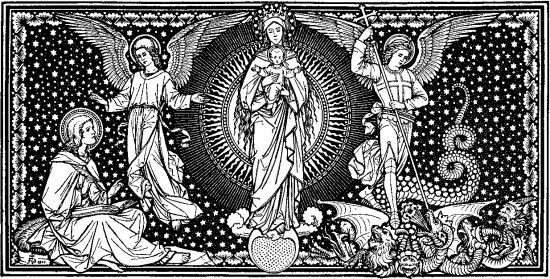
\includegraphics[width=1.0\textwidth]{maria_virgo_mater2.jpg}
	\vfill
	\tytulfont{DOMINICA\\AD VESPERAS}
	\vfill
	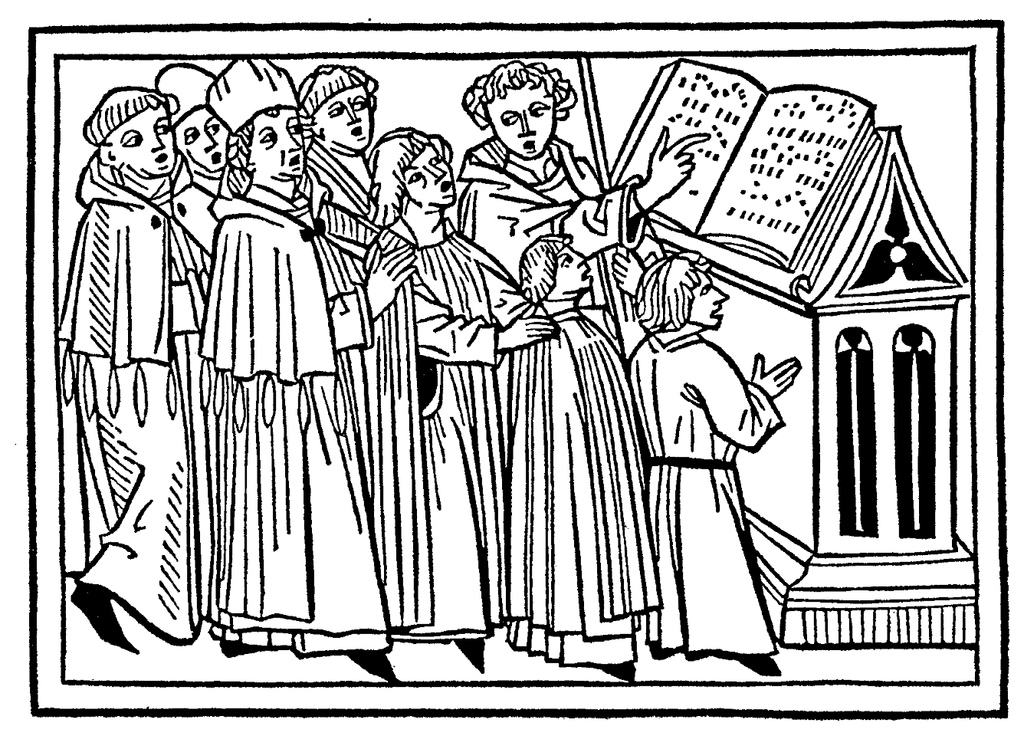
\includegraphics[width=0.6\textwidth]{singers_okładka.jpg}
\end{center}%
% <c><v>*</v></c>
% <c><v>†</v></c>
% <c><i>Ps.</i></c> 
% <c><sp>V/</sp>.</c>
% <c><i>ij.</i></c>
% \noindent\hrulefill \red{†}~ \red{*}~ 
% é á í ó ú ý æ ǽ œ Á, É, Í, Ó, Ú, Ý Æ Ǽ Œ \'{\oe} \'{\OE}
% \tikz[overlay]\draw[red](-10,0)--++(15,0);
% \fsize \the\baselineskip - czcionka i odstęp
\pagebreak
\thispagestyle{empty}
\sekcja{Ante Divinum officium}{Odmawia się po cichu w pozycji klęczącej kreśląc znak krzyża na ustach.}%
\BeginParallel{0.5}
	\latN{\inicjal{A}{péri},~\red{\grecross}~Dómine, méum ad benedicéndum nómen sánctum túum: múnda quoqúe cor méum ab ómnibus vánis, pervérsis et aliénis cogitatiónibus; intelléctum illúmina, afféctum inflámma, ut dígne, atténte ac devóte hoc Offícium recitáre váleam, et exaudíri mérear ánte conspéctum divínae Majestátis túae. Per Chrístum Dóminum nóstrum. Amen.\linespace}
	\polN{\inicjal{O}{twórz},~\red{\grecross}~Panie, usta moje, dla błogosławienia świętego imienia Twego: oczyść także serce moje od wszelkich myśli próżnych, przewrotnych i~niewłaściwych; oświeć rozum, rozpal uczucie, abym godnie, uważnie i~pobożnie mógł odmówić to oficjum, i~zasłużył na wysłuchanie przed obliczem Twego Boskiego majestatu. Przez Chrystusa, Pana naszego. Amen.\linespace}
 	\latN{\inicjal{D}{ómine}, in unióne illíus divínae intentiónis, qúa ípse in térris laúdes Déo persolvísti, hanc tíbi Hóram persólvo.}
	\polN{\inicjal{P}{anie}, w~zjednoczeniu z~tą Boską intencją, z~którą Ty sam, na ziemi będąc, chwałę Bogu zanosiłeś, Tobie te godziny zanoszę.}
\EndParallel
\dekor{0.4}{benedicamus_domino.jpg}
\pagebreak
\setcounter{page}{1}
\fancyhead{}% wyczyść wszystkie pola nagłówka
\pagestyle{plain}% nagłówek i stopka pusta - UWAGA: przedefiniowany styl przez polecenie fancypagestyle w header.tex	
\gresetbracerendering{font}%
%% -----------------  INCIPIT ---------------------
\pasek{1.0}{pasek-incipit-10mm.jpg}
\sectionspace%
\gresetinitiallines{0}\gabcsnippet{(c3) <c><sp>V/</sp>.</c> De([alt:Hebdomadarius]h)us(h'_) <c><v>\grecross</v></c> (,) in(h) ad(h)ju(h)tó(i)ri(h)um(h) me(h)um(h'_) in(h)tén(g)de.(h.) (::) <c><sp>R/</sp>.</c> Dó([alt:Chorus]h)mi(h)ne(h'_) (,) ad(h) ad(h)ju(h)ván(h)dum(h) me(h'_) fe(h)stí(g)na.(h.) (:) Gló(h)ri(h)a(h) Pa(h)tri,(h) et(h) Fí(h)li(h)o,(h'_) (,) et(h) Spi(h)rí(h)tu(h)i(h) San(g)cto.(h.) (:) Sic(h)ut(h) e(h)rat(h) in(h) prin(h)cí(h)pi(h)o,(h) et(h) nunc,(h) et(h) sem(h)per,(h.) (,) et(h) in(h) saé(h)cu(h)la(h) sae(h)cu(h)ló(h)rum.(h) A(g)men.(h.) (;) Al(h)le(i)lú(hg~){ia}.(g.) (::) (z-) <alt>A Septuagesima usque ad Pascha, loco Alleluia, dicitur :</alt> Laus(h) ti(h)bi(h) Dó(h)mi(h)ne(h'_) Rex(h) ae(h)tér(h)nae(i) gló(h')ri(h)ae.(g.) (::)}\linespace
\tlumaczR{\red{\Vbar.}~Boże, \red{\grecross}~wejrzyj ku wspomożeniu memu. \red{\Rbar.}~Panie, pośpiesz ku ratunkowi memu. Chwała Ojcu i Synowi, i Duchowi Święte-\\mu. Jak była na początku, teraz i zawsze, i na wieki wieków. Amen. Alleluja.~\emph{/}~Chwała Tobie Panie, Królu wiecznej chwały.}
\dekor{0.45}{amdg02.jpg}
\pagebreak
%% -----------------  PSALMI ---------------------
\pasek{1.0}{pasek-psalmi-10mm.jpg}
\sectionspace\sectionspace%
\gresetinitiallines{1}\greannotation{1. Ant.}\greannotation{7. c2}\gabcsnippet{(c3) DI([alt:Hebdomadarius]g)xit(h) Dó(i)mi(j)nus.(i.) (::) Dó(k)mi([alt:Cantor]j)no(j) me(i)o(j.) : <c><v>*</v></c> (;) Se([alt:Chorus]i)de(i) a(i) dex(j)tris(i) me(h)is.(ih..) (::)}\linespace
\tlumaczR{Rzekł Pan \red{‡} Panu memu:~\red{*} Siądź po prawicy mojej:}%
\segmentspace
%% --- 1. Psalm 109 - 1 g------<c><v>\greheightstar</v></c>
\subsekcja{Psalm 109}
\vspace{-10pt}
\gresetinitiallines{0}\greannotation{Psalm}\greannotation{109}\gabcsnippet{(c3)<c><v>\footnotesize{2.  }</v></c>Dó(i)nec(i) pó(i)nam(i) in(i)i(i)<b>mí</b>(k)cos(j) <b>tú</b>(i)os,(j.) ~<c><v>*</v></c>(:) sca(i)bél(i)lum(i) <b>pé</b>(j)dum(i) tu(i)<b>ó</b>(h)rum.(ih..) (::)}\linespace
\tlumaczR{Aż położę nieprzyjaciół twoich,~\red{*} podnóżkiem nóg twoich.}\
\BeginParallel{0.7}
\latNPs{\mred{3.}~Vírgam virtútis túae emíttet Dómi\textbf{nus} ex \textbf{Sí}on:~\red{*} domináre in médio inimi\textbf{có}rum tu\textbf{ó}rum.}\polPs{Berło mocy twojej wypuści Pan z Syjonu:~\red{*} panuj wpośród nieprzyjaciół twoich.}%
\latNPs{\mred{4.}~Técum princípium in díe virtútis túae in splendóri\textbf{bus} sanc\textbf{tó}rum:~\red{*} ex útero ánte lucíferum \textbf{gé}nu\textbf{i} te.}\polPs{Przy tobie panowanie w dzień mocy twej w blaskach świętości:~\red{*} z żywota przed jutrzenką zrodziłem cię.}%
\latNPs{\mred{5.}~Jurávit Dóminus, et non poeni\textbf{té}bit \textbf{é}um:~\red{*} Tu es sacérdos in aetérnum secúndum órdi\textbf{nem} Mel\textbf{chí}sedech.}\polPs{Przysiągł Pan i nic będzie żałował:~\red{*} Ty jesteś kapłanem na wieki, według porządku Melchizedecha.}%
\latNPs{\mred{6.}~Dóminus a \textbf{déx}tris \textbf{tú}is,~\red{*} confrégit in díe iráe su\textbf{á}e \textbf{ré}ges.}\polPs{Pan po prawicy twojej,~\red{*} poraził w dzień gniewu swego królów.}%
\latNPs{\mred{7.}~Judicábit in natiónibus, im\textbf{plé}bit ru\textbf{í}nas:~\red{*} conquassábit cápita in \textbf{tér}ra mul\textbf{tó}rum.}\polPs{Będzie sądził narody, dopełni zagłady,~\red{*} potłucze głowy wielu na ziemi.}%
\latNPs{\mred{8.}~De torrénte in \textbf{ví}a \textbf{bí}bet:~\red{*} proptérea exal\textbf{tá}bit \textbf{cá}put.}\polPs{Ze strumienia na drodze pić będzie:~\red{*} dlatego wywyższy głowę.}%
\latNPs{\mred{9.}~Glória \textbf{Pá}tri, et \textbf{Fí}lio,~\red{*} et Spi\textbf{rí}tui \textbf{Sánc}to.}\polPs{Chwała Ojcu i Synowi,~\red{*} i Duchowi Świętemu.}%
\latNPs{\mred{10.}~Sicut érat in princípio, et \textbf{nunc}, et \textbf{sém}per,~\red{*} et in saécula saecu\textbf{ló}rum. \textbf{A}men.}\polPs{Jak była na początku, teraz i zawsze,~\red{*} i na wieki wieków. Amen.}%
\EndParallel
\paragraphspace
\gresetinitiallines{1}\greannotation{1. Ant.}\greannotation{7. c2}\gabcsnippet{(c3) DI(g)xit(h) Dó(i)mi(j)nus(i.) (,) Dó(i_[oh:h]h)mi(f)no(h) me(g_[oh:h]f)o :(e.) (;) Se(f)de(f') a(d) dex(fh)tris(g) me(e.)is.(e.) (::)}\linespace
\tlumaczR{Rzekł Pan Panu memu: Siądź po prawicy mojej:}
\pagebreak
%% --- 2. Psalm 110 - 2D ---[alt:fit reverentia]
\gresetinitiallines{1}\greannotation{2. Ant.}\greannotation{3. b}\gabcsnippet{(c4) MA(g_[uh:l]j)gna(ji) ó(h')pe(g)ra(h') Dó(i)mi(hg)ni,(g.) (::)}
\vspace{-14pt}
\tlumaczR{Wielkie sprawy Pańskie:}%
\subsekcja{Psalm 110}
\vspace{-10pt}
\gresetinitiallines{0}\greannotation{Psalm}\greannotation{110}\gabcsnippet{(c4)<c><v>\footnotesize{1.  }</v></c>Con(g)fi(hj)té(j)bor(j) tí(j)bi,(j) Dó(j)mi(j)ne,(j) in(j) tó(j)to(j) <b>cór</b>(k jr)de(j jr[ocb:1{]) <b>mé</b>(ih[ocb:0}])o:(j.) ~<c><v>*</v></c>(:) in(j) con(j)sí(j)li(j)o(j) jus(j)tó(j)rum,(j) et(j) con(j)gre(j)ga(j)<ul><i>ti</i></ul>(h)<b>ó</b>(j jr)ne.(i.) (::) ()<c><i><v>\footnotesize{Flex:}</v></i></c>() su(j)ó(j)rum,(h.) <c><v>†</v></c>(::)}
\vspace{-24pt}
\tlumaczR{Będę Cię wysławiał, Panie wszystkim sercem moim,~\red{*}\\w radzie sprawiedliwych i w zgromadzeniu.}%
\linespace
\BeginParallel{0.7}
\latNPs{\mred{2.}~Mágna \textbf{ó}pera \textbf{Dó}\textbf{mi}ni:~\red{*} exquisíta in ómnes voluntá\underline{\textit{tes}} \textbf{é}jus.}\polPs{Wielkie są dzieła Pańskie,~\red{*} doświadczone według wszystkiego upodobania Jego.}%
\latNPs{\mred{3.}~Conféssio et magnificéntia \textbf{ó}pus \textbf{é}jus:~\red{*} et justítia éjus mánet in sǽcu\underline{\textit{lum}} \textbf{sǽ}culi.}\polPs{Chwalebne i wspaniałe jest dzieło Jego,~\red{*} a sprawiedliwość Jego trwa na wieki wieków.}%

\latNPs{\mred{4.}~Memóriam fécit mirabílium suórum,~\red{†} miséricors et mise\textbf{rá}tor \textbf{Dó}\textbf{mi}nus:~\red{*} éscam dédit timén\underline{\textit{ti}}\textbf{bus} se.}\polPs{Uczynił pamiątkę dziwów swoich miłosierny~\red{†} i litościwy Pan:~\red{*} dał pokarm tym, którzy się Go boją.}%
\latNPs{\mred{5.}~Mémor érit in sǽculum testa\textbf{mén}ti \textbf{sú}i:~\red{*} virtútem óperum suórum annuntiábit pópulo súo:}\polPs{Pamiętać będzie wiecznie na przymierze swoje:~\red{*} moc uczynków swoich oznajmi ludowi swemu:}%
\latNPs{\mred{6.}~Ut det íllis heredi\textbf{tá}tem \textbf{gén}\textbf{ti}um:~\red{*} ópera mánuum éjus véritas, et \underline{\textit{ju}}\textbf{dí}cium.}\polPs{Aby im dać dziedzictwo narodów:~\red{*} dzieła rąk Jego są prawdą i sądem.}%
\latNPs{\mred{7.}~Fidélia ómnia mandáta éjus:~\red{†} confirmáta in \textbf{sǽ}culum \textbf{sǽ}\textbf{cu}li,~\red{*} fácta in veritáte et ae\underline{\textit{qui}}\textbf{tá}te.}\polPs{Pewne są wszystkie przykazania Jego,~\red{†} utwierdzone na wieki wieków,~\red{*} uczynione w prawdzie i w prawości.}%
\latNPs{\mred{8.}~Redemptiónem mísit \textbf{pó}pulo \textbf{sú}o:~\red{*} mandávit in aetérnum testamén\underline{\textit{tum}} \textbf{sú}um.}\polPs{Zesłał odkupienie ludowi swemu,~\red{*} ustanowił na wieki przymierze swoje.}%
\latNPs{\mred{9.}~\red{\footnotesize{Fit reverentia}} Sánctum, et terríbile \textbf{nó}men \textbf{é}jus:~\red{*} inítium sapiéntiae tí\underline{\textit{mor}} \textbf{Dó}mini.}\polPs{Święte i straszne jest imię Jego:~\red{*} początkiem mądrości jest bojaźń Pańska.}%
\latNPs{\mred{10.}~Intelléctus bónus ómnibus faci\textbf{én}tibus \textbf{é}um:~\red{*} laudátio éjus mánet in sǽcu\underline{\textit{lum}} \textbf{sǽ}culi.}\polPs{Zrozumienie dobre mają, wszyscy, którzy tak czynią:~\red{*} chwała Jego trwa na wieki wieków.}%
\latNPs{\mred{11.}~Glória \textbf{Pá}tri, et \textbf{Fí}\textbf{li}o,~\red{*} et Spirítu\underline{\textit{i}} \textbf{Sánc}to.}\polPs{Chwała Ojcu i Synowi,~\red{*} i Duchowi Świętemu.}%
\latNPs{\mred{12.}~Sicut érat in princípio, et \textbf{nunc}, et \textbf{sém}per,~\red{*} et in saécula saeculó\underline{\textit{rum}}. \textbf{A}men.}\polPs{Jak była na początku, teraz i zawsze,~\red{*} i na wieki wieków. Amen.}%
\EndParallel
\linespace
\gresetinitiallines{1}\greannotation{2. Ant.}\greannotation{3. b}\gabcsnippet{(c4) MA(g_[uh:l]j)gna(ji) ó(h')pe(g)ra(h') Dó(i)mi(hg)ni,(g.) (;) ex(h)qui(g)sí(e_0[uh:l]fg)ta(g') in(e) o(f')mnes(d) vo(e')lun(f)tá(g_[uh:l]h)tes(gf) e(e.)jus.(e.) (::)}%
\linespace
\tlumaczR{Wielkie sprawy Pańskie: doświadczone we wszystkiem upodobaniu jego.}%
\pagebreak
%% --- 3. Psalm 111 - 3a ---
\gresetinitiallines{1}\greannotation{3. Ant.}\greannotation{4. G}\gabcsnippet{(c4) Qui(g) ti(e')met(f) Dó(g)mi(h)num,(g'_) <c><v>*</v></c>(,) in(g) man(gh)dá(h)tis(g') e(g)jus(e_f) cu(gf)pit(de) ni(e.)mis.(e.) (::)}
\linespace
\subsekcja{Psalm 111}
\vspace{-10pt}
\gresetinitiallines{0}\greannotation{Psalm}\greannotation{111}\gabcsnippet{(c4)<c><v>\footnotesize{1.  }</v></c>Be(h)á(gh)tus(h) vír,(h) qú(h)i(h) <i>tí</i>(g)<i>met</i>(h) <b>Dó</b>(i)mi(hr)num:(h.) ~<c><v>*</v></c>(:) in(h) man(h)dá(h)tis(h) é(h)jus(h) vó(h)let(h) <b>ní</b>(h gr)mis.(g.) (::)
()<c><i><v>\footnotesize{Flex:}</v></i></c>()  cóm(h)mo(g)dat,(g.) (::)}
\BeginParallel{0.7}
\latNPs{\mred{2.}~Pótens in térra érit \underline{\textit{sé}}\underline{\textit{men}} \textbf{é}jus:~\red{*} generátio rectórum benedi\textbf{cé}tur.}\polPs{}%
\latNPs{\mred{3.}~Glória, et divítiae in \underline{\textit{dó}}\underline{\textit{mo}} \textbf{é}jus:~\red{*} et justítia éjus mánet in sǽculum \textbf{sǽ}culi.}\polPs{}%
\latNPs{\mred{4.}~Exórtum est in ténebris \underline{\textit{lú}}\underline{\textit{men}} \textbf{réc}tis:~\red{*} miséricors, et miserátor, et \textbf{jús}tus.}\polPs{}%
\latNPs{\mred{5.}~Jucúndus hómo qúi miserétur et cómmodat,~\red{†} dispónet sermónes súos \underline{\textit{in}} \underline{\textit{ju}}\textbf{dí}cio:~\red{*} }\polPs{}%
\latNPs{\mred{6.}~In memória aetérna \underline{\textit{é}}\underline{\textit{rit}} \textbf{jús}tus:~\red{*} ab auditióne mála non ti\textbf{mé}bit.}\polPs{}%
\latNPs{\mred{7.}~Parátum cor éjus speráre in Dómino,~\red{†} confirmátum \underline{\textit{est}} \underline{\textit{cor}} \textbf{é}jus:~\red{*} non commovébitur dónec despíciat inimícos \textbf{sú}os.}\polPs{}%
\latNPs{\mred{8.}~Dispérsit, dédit paupéribus:~† justítia éjus mánet in sǽ\underline{\textit{cu}}\underline{\textit{lum}} \textbf{sǽ}culi,~\red{*} córnu éjus exaltábitur in \textbf{gló}ria.}\polPs{}%
\latNPs{\mred{9.}~Peccátor vidébit, et irascétur,~† déntibus súis frémet \underline{\textit{et}} \underline{\textit{ta}}\textbf{bé}scet:~\red{*} desidérium peccatórum per\textbf{í}bit.}\polPs{}%
\latNPs{\mred{10.}~Glória Pá\underline{\textit{tri}}, \underline{\textit{et}} \textbf{Fí}lio,~\red{*} et Spirítui \textbf{Sánc}to.}\polPs{}%
\latNPs{\mred{11.}~Sicut érat in princípio, et \underline{\textit{nunc}}, \underline{\textit{et}} \textbf{sém}per,~\red{*} et in saécula saeculórum. \textbf{A}men.}\polPs{}%
\EndParallel
\gresetinitiallines{1}\greannotation{3. Ant.}\greannotation{4. G}\gabcsnippet{(c4) Qui(g) ti(e')met(f) Dó(g)mi(h)num,(g'_) (,) in(g) man(gh)dá(h)tis(g') e(g)jus(e_f) cu(gf)pit(de) ni(e.)mis.(e.) (::)}
\paragraphspace
%% --- 4. Psalm 112 - 4E ---
\gresetinitiallines{1}\greannotation{4. Ant.}\greannotation{7. C}\gabcsnippet{(c3) SIT(ii) no(g)men(h) Dó(ij)mi(i)ni(h.) <c><v>*</v></c>(,) be(hg)ne(f)dí(g_[uh:l]h)ctum(ih) in(f) saé(e')cu(e)la.(e.) (::)}
\linespace
\subsekcja{Psalm 112}
\vspace{-10pt}
\gresetinitiallines{0}\greannotation{Psalm}\greannotation{112}\gabcsnippet{(c3) <c><v>\footnotesize{1.  }</v></c>Lau(hg)dá(hi)te,(i) <b>pú</b>(k)e(jr)ri,(j) <b>Dó</b>(i)mi(jr)num:(j.) ~<c><v>*</v></c>(:) lau(i)dá(i)te(i) <b>nó</b>(j ir)men(i) <b>Dó</b>(h)mi(hr)ni.(gh..) (::)}
\BeginParallel{0.7}
\latNPs{\mred{2.}~(fit reverentía) Sit nómen Dómini \textbf{be}ne\textbf{díc}tum,~\red{*} ex hoc nunc, et \textbf{usqú}e in \textbf{sǽ}culum.}\polPs{}%
\latNPs{\mred{3.}~A sólis órtu usqúe \textbf{ad} oc\textbf{cá}sum,~\red{*} laudábile \textbf{nó}men \textbf{Dó}mini.}\polPs{}%
\latNPs{\mred{4.}~Excélsus súper ómnes \textbf{gén}tes \textbf{Dó}minus,~\red{*} et súper caélos \textbf{gló}ria \textbf{é}jus.}\polPs{}%
\latNPs{\mred{5.}~Qúis sícut Dóminus, Déus nóster, qúi in \textbf{ál}tis \textbf{há}bitat,~\red{*} }\polPs{}%
\latNPs{\mred{6.}~Súscitans a \textbf{tér}ra \textbf{ín}opem,~\red{*} et de stércore \textbf{é}rigens \textbf{páu}perem:}\polPs{}%
\latNPs{\mred{7.}~Ut cóllocet éum \textbf{cum} prin\textbf{cí}pibus,~\red{*} cum princípibus \textbf{pó}puli \textbf{sú}i.}\polPs{}%
\latNPs{\mred{8.}~Qúi habitáre fácit stéri\textbf{lem} in \textbf{dó}mo,~\red{*} mátrem filiórum \textbf{la}e\textbf{tán}tem.}\polPs{}%
\latNPs{\mred{9.}~Glória \textbf{Pá}tri, et \textbf{Fí}lio,~\red{*} et Spi\textbf{rí}tui \textbf{Sánc}to.}\polPs{}%
\latNPs{\mred{10.}~Sicut érat in princípio, et \textbf{nunc}, et \textbf{sém}per,~\red{*} et in saécula saecu\textbf{ló}rum. \textbf{A}men.}\polPs{}%
\EndParallel
\linespace
\gresetinitiallines{1}\greannotation{4. Ant.}\greannotation{4. E}\gabcsnippet{(c3) SIT(ii) no(g)men(h) Dó(ij)mi(i)ni(h.) (,) be(hg)ne(f)dí(g_[uh:l]h)ctum(ih) in(f) saé(e')cu(e)la.(e.) (::)}
\paragraphspace
%% --- 5. Psalm 113 - PER ---
\gresetinitiallines{1}\greannotation{5. Ant.}\greannotation{PER}\gabcsnippet{(c4) De(c')us(d) au(f')tem(e) no(fg)ster(g) in(gh) cae(fe)lo:(d.) <c><v>*</v></c>(;) ó(f')mni(g)a(h') quae(ixi)cúm(h)que(gf) vó(g')lu(f)it,(gh) fe(g.)cit.(g.) (::)}
\linespace
\subsekcja{Psalm 113}
\vspace{-10pt}
\gresetinitiallines{0}\greannotation{Psalm}\greannotation{113}\gabcsnippet{(c4)<c><v>\footnotesize{1.  }</v></c>In(ixhi) éx(h)i(h)tu(h) Is(h)ra(h)ël(h) <i>de</i>(g) <i>A</i>(ixi)<i>e</i>(h)<b>gýp</b>(g fr)to,(f.) ~<c><v>*</v></c>(:) dó(g)mus(g) Já(g)cob(g) de(g) pó(g)pu(g)<i>lo</i>(d) <b>bár</b>(f)ba(fr)ro:(ed..) (::)
<i>Flex:</i>()  pal(h)pá(h)bunt: <c><v>†</v></c>(g. h h h  ::)}
\BeginParallel{0.7}
\latNPs{\mred{2.}~Fácta est Judǽa sanctifi\underline{\textit{cá}}\underline{\textit{ti}}\underline{\textit{o}} \textbf{é}jus,~\red{*} Israël potés\underline{\textit{tas}} \textbf{é}jus.}\polPs{}%
\latNPs{\mred{3.}~Máre \underline{\textit{ví}}\underline{\textit{dit}}, \underline{\textit{et}} \textbf{fú}git:~\red{*} Jordánis convérsus est \underline{\textit{re}}\textbf{trór}sum.}\polPs{}%
\latNPs{\mred{4.}~Móntes exsultavé\underline{\textit{runt}} \underline{\textit{ut}} \underline{\textit{a}}\textbf{rí}etes,~\red{*} et cólles sícut á\underline{\textit{gni}} \textbf{ó}vium.}\polPs{}%
\latNPs{\mred{5.}~Qúid est tíbi, máre, \underline{\textit{qú}}\underline{\textit{od}} \underline{\textit{fu}}\textbf{gís}ti:~\red{*} et tu, Jordánis, quía convérsus es \underline{\textit{re}}\textbf{trór}sum?}\polPs{}%
\latNPs{\mred{6.}~Móntes, exsultástis \underline{\textit{síc}}\underline{\textit{ut}} \underline{\textit{a}}\textbf{rí}etes,~\red{*} et cólles, sícut á\underline{\textit{gni}} \textbf{ó}vium.}\polPs{}%
\latNPs{\mred{7.}~A fácie Dómini \underline{\textit{mó}}\underline{\textit{ta}} \underline{\textit{est}} \textbf{tér}ra,~\red{*} a fácie Dé\underline{\textit{i}} \textbf{Já}cob.}\polPs{}%
\latNPs{\mred{8.}~Qúi convértit pétram in \underline{\textit{stá}}\underline{\textit{gna}} \underline{\textit{a}}\textbf{quá}rum,~\red{*} et rúpem in fóntes \underline{\textit{a}}\textbf{quá}rum.}\polPs{}%
\latNPs{\mred{9.}~Non nóbis, Dó\underline{\textit{mi}}\underline{\textit{ne}}, \underline{\textit{non}} \textbf{nó}bis:~\red{*} sed nómini túo \underline{\textit{da}} \textbf{gló}riam.}\polPs{}%
\latNPs{\mred{10.}~Súper misericórdia túa, et ve\underline{\textit{ri}}\underline{\textit{tá}}\underline{\textit{te}} \textbf{tú}a:~\red{*} nequándo dícant géntes: Ubi est Déus \underline{\textit{e}}\textbf{ó}rum?}\polPs{}%
\latNPs{\mred{11.}~Déus áutem nós\underline{\textit{ter}} \underline{\textit{in}} \underline{\textit{ca}}\textbf{é}lo:~\red{*} ómnia quaecúmque vólu\underline{\textit{it}}, \textbf{fé}cit.}\polPs{}%
\latNPs{\mred{12.}~Simulácra géntium argén\underline{\textit{tum}}, \underline{\textit{et}} \underline{\textit{a}}\textbf{ú}rum,~\red{*} ópera mánu\underline{\textit{um}} \textbf{hó}minum.}\polPs{}%
\latNPs{\mred{13.}~Os hábent, \underline{\textit{et}} \underline{\textit{non}} \underline{\textit{lo}}\textbf{quén}tur:~\red{*} óculos hábent, et non \underline{\textit{vi}}\textbf{dé}bunt.}\polPs{}%
\latNPs{\mred{14.}~Aúres há\underline{\textit{bent}}, \underline{\textit{et}} \underline{\textit{non}} \textbf{áu}dient:~\red{*} náres hábent, et non o\underline{\textit{do}}\textbf{rá}bunt.}\polPs{}%
\latNPs{\mred{15.}~Mánus hábent, et non palpábunt:~† pédes hábent, et \underline{\textit{non}} \underline{\textit{am}}\underline{\textit{bu}}\textbf{lá}bunt:~\red{*} non clamábunt in gúttu\underline{\textit{re}} \textbf{sú}o.}\polPs{}%
\latNPs{\mred{16.}~Símiles íllis fíant qúi \underline{\textit{fá}}\underline{\textit{ci}}\underline{\textit{unt}} \textbf{é}a:~\red{*} et ómnes qúi confídunt \underline{\textit{in}} \textbf{é}is.}\polPs{}%
\latNPs{\mred{17.}~Dómus Israël spe\underline{\textit{rá}}\underline{\textit{vit}} \underline{\textit{in}} \textbf{Dó}mino:~\red{*} adjútor eórum et protéctor \underline{\textit{e}}\textbf{ó}rum est,}\polPs{}%
\latNPs{\mred{18.}~Dómus Aáron spe\underline{\textit{rá}}\underline{\textit{vit}} \underline{\textit{in}} \textbf{Dó}mino:~\red{*} adjútor eórum et protéctor \underline{\textit{e}}\textbf{ó}rum est,}\polPs{}%
\latNPs{\mred{19.}~Qúi tíment Dóminum, spera\underline{\textit{vé}}\underline{\textit{runt}} \underline{\textit{in}} \textbf{Dó}mino:~\red{*} adjútor eórum et protéctor \underline{\textit{e}}\textbf{ó}rum est.}\polPs{}%
\latNPs{\mred{20.}~Dóminus mé\underline{\textit{mor}} \underline{\textit{fú}}\underline{\textit{it}} \textbf{nós}tri:~\red{*} et benedí\underline{\textit{xit}} \textbf{nó}bis:}\polPs{}%
\latNPs{\mred{21.}~Benedíxit \underline{\textit{dó}}\underline{\textit{mu}}\underline{\textit{i}} \textbf{Is}raël:~\red{*} benedíxit dómui \underline{\textit{A}}\textbf{á}ron.}\polPs{}%
\latNPs{\mred{22.}~Benedíxit ómnibus, qú\underline{\textit{i}} \underline{\textit{tí}}\underline{\textit{ment}} \textbf{Dó}minum,~\red{*} pusíllis cum \underline{\textit{ma}}\textbf{jó}ribus.}\polPs{}%
\latNPs{\mred{23.}~Adíciat \underline{\textit{Dó}}\underline{\textit{mi}}\underline{\textit{nus}} \textbf{sú}per vos:~\red{*} súper vos, et súper fíli\underline{\textit{os}} \textbf{vés}tros.}\polPs{}%
\latNPs{\mred{24.}~Benedíc\underline{\textit{ti}} \underline{\textit{vos}} \underline{\textit{a}} \textbf{Dó}mino,~\red{*} qúi fécit caélum, \underline{\textit{et}} \textbf{tér}ram.}\polPs{}%
\latNPs{\mred{25.}~Caélum \underline{\textit{ca}}\underline{\textit{é}}\underline{\textit{li}} \textbf{Dó}mino:~\red{*} térram áutem dédit fíli\underline{\textit{is}} \textbf{hó}minum.}\polPs{}%
\latNPs{\mred{26.}~Non mórtui lau\underline{\textit{dá}}\underline{\textit{bunt}} \underline{\textit{te}}, \textbf{Dó}mine:~\red{*} néque ómnes, qúi descéndunt in \underline{\textit{in}}\textbf{fér}num.}\polPs{}%
\latNPs{\mred{27.}~Sed nos qúi vívimus, bene\underline{\textit{dí}}\underline{\textit{ci}}\underline{\textit{mus}} \textbf{Dó}mino,~\red{*} ex hoc nunc et usqúe \underline{\textit{in}} \textbf{sǽ}culum.}\polPs{}%
\latNPs{\mred{28.}~Glória \underline{\textit{Pá}}\underline{\textit{tri}}, \underline{\textit{et}} \textbf{Fí}lio,~\red{*} et Spirítu\underline{\textit{i}} \textbf{Sánc}to.}\polPs{}%
\latNPs{\mred{29.}~Sicut érat in princípio, \underline{\textit{et}} \underline{\textit{nunc}}, \underline{\textit{et}} \textbf{sém}per,~\red{*} et in saécula saeculó\underline{\textit{rum}}. \textbf{A}men.}\polPs{}%
\EndParallel
\gresetinitiallines{1}\greannotation{5. Ant.}\greannotation{PER}\gabcsnippet{(c4) De(c')us(d) au(f')tem(e) no(fg)ster(g) in(gh) cae(fe)lo:(d.) (;) ó(f')mni(g)a(h') quae(ixi)cúm(h)que(gf) vó(g')lu(f)it,(gh) fe(g.)cit.(g.) (::)}
\sectionspace
%% --- Capitulum---
\pasek{1.0}{pasek-capitulum-10mm.jpg}
\sectionspace\paragraphspace%
\gresetinitiallines{1}\grecommentary{2 Cor 1,3-4}\gabcsnippet{(c3)Be([alt:Hebdomadarius]h)ne(h)dí(h)ctus(h) De(h)us,(h) et(h) Pa(h)ter(h) Dó(h)mi(h)ni(h) no(h)stri(h) Ie(h)su(h) Chri(h)sti,(f.)  <c><v>†</v></c>(,)  Pa(h)ter(h) mi(h)se(h)ri(h)cor(h)di(h)á(h)rum,(h) et(h) De(h)us(h) to(h)tí(h)us(h) con(h)so(h)la(f)ti(e)ó(h)nis,(h)  <c><v>*</v></c>(;)  qui(h) con(h)so(h)lá(h)tur(h) nos(h) in(h) o(h)mni(h) tri(h)bu(h)la(h)ti(h)ó(h)ne(f) no(e)stra.(e.f.)   <c><sp>R/</sp>.</c>(::)}\linespace
\gresetinitiallines{0}\gabcsnippet{(c3) <c><sp>R/</sp>.</c> De(h)o(h) grá(f)ti(e)as.(e.f.) (::)}
\vspace{-26pt}
\tlumaczR{TBłogosławiony Bóg i Ojciec Pana naszego Jezusa Chrystusa, Ojciec miłosierdzia, a Bóg wszystkiéj pociechy, który nas cieszy we wszelakiem utrapieniu naszem.}
\sectionspace
%% --- Hymnus ---
\pasek{1.0}{pasek-hymnus-10mm.jpg}
\gresetinitiallines{1}\greannotation{Hymn.}\greannotation{8.}\gabcsnippet{(c3) LU(e)cis(fh) Cre(h)á(hg)tor(fe) óp(h)ti(i)me,(gvFE.) (,) Lu(hi)cem(jh) di(i)é(hvGF')rum(g) pró(g')fe(f)rens,(e.) (;) Pri(e)mór(fh)di(h)is(hg) lu(fe)cis(h) no(i)vae(gvFE.) (,) Mun(hi)di(jh) pa(i)rans(hf) o(g)rí(fg)gi(f)nem:(e.) 2.(::) Qui(e) ma(fh)ne(h) jun(hg)ctum(fe) vé(h)spe(i)ri(gvFE.) (,) Di(hi)em(jh) vo(i)cá(hvGF')ri(g) praé(g')ci(f)pis:(e.) (;) Il(e)lá(fh)bi(h)tur(hg) te(fe)trum(h) cha(i)os,(gvFE.) (,) Au(hi)di(jh) pre(i)ces(hf) cum(g) flé(fg)ti(f)bus.(e.) 3.(::) Ne(e) mens(fh) gra(h)vá(hg)ta(fe) crí(h)mi(i)ne,(gvFE.) (,) Vi(hi)tae(jh) sit(i) ex(hvGF')sul(g) mú(g')ne(f)re,(e.) (;) Dum(e) nil(fh) pe(h)rén(hg)ne(fe) có(h)gi(i)tat,(gvFE.) (,) Se(hi)sé(jh)que(i) cul(hf)pis(g) íl(fg)li(f)gat.(e.) 4.(::) Cae(e)lé(fh)ste(h) pul(hg)set(fe) ó(h)sti(i)um,(gvFE.) (,) Vi(hi)tá(jh)le(i) tol(hvGF')lat(g) praé(g')mi(f)um:(e.) (;) Vi(e)té(fh)mus(h) o(hg)mne(fe) nó(h)xi(i)um,(gvFE.) (,) Pur(hi)gé(jh)mus(i) o(hf)mne(g) pés(fg)si(f)mum.(e.) 5.(::) Prae(e)sta,(fh) Pa(h)ter(hg) pi(fe)ís(h)si(i)me,(gvFE.) (,) Pa(hi)trí(jh)que(i) com(hvGF')par(g) U(g')ni(f)ce,(e.) (;) Cum(e) Spí(fh)ri(h)tu(hg) Pa(fe)rá(h)cli(i)to,(gvFE.) (,) Re(hi)gnans(jh) per(i) o(hf)mne(g) saé(fg)cu(f)lum.(e.) (::) A(efe)men.(de..) (::)}\linespace
\tlumacz{\red{1.}~Najlepszy Stwórco światła, Który tworzysz światło dni Początkami nowego światła Sprawiasz powstanie świata: \red{2.}~Który ranek, złączony z wieczorem, Każesz nazywać dniem, Wysłuchaj, gdy ogarnia ciemna otchłań, Modlitw płaczących. \red{3.}~By dusza winą obarczona, Nie była pozbawiona daru żywota, Gdy nie myśląc nie przemija, Wikła się w grzechach. \red{4.}~Niech zapuka do bramy niebieskiej Weźmie nagrodę żywota; Unikajmy grzechu każdego, Zmywajmy wszelką winę. \red{5.}~Udziel Ojcze najmiłościwszy, I Ty Jedyny równy Ojcu, Z Duchem Pocieszycielem Królujący po wszystek wiek. Amen.}
\sectionspace
%% --- Versus - Respons (simple)--- .
\sekcja{Versus}{}
\gresetinitiallines{0}\gabcsnippet{(c4)  <c><sp>V/</sp>.</c>() Di(h)ri(h)gá(h)tur,(h) Dó(h)mi(h)ne(h) ,()oráti(h)ome(h)a.(g'_//hvGF'E/fgf.) (::)}
\hspace{2pt}\red{\Rbar.}~Sicut incénsum in conspéctutu-o.\linespace
\sectionspace
%% --- End Versus - Respons (simple)---
%\includegraphics[width=1.0\textwidth]{visitatio02.jpg}
%% --- Magnificat ---ó á é ú í <c><v>\grecross</v></c> <c><v>\greheightstar</v></c>
\pasek{1.0}{pasek-canticum-10mm.jpg}
\sectionspace%
\gresetinitiallines{1}\greannotation{Ant. Magn.}\greannotation{1. G}\gabcsnippet{(c4) COl(cd)lí(ixdh'!iv)gi(h')te(h) <c><v>*</v></c>(,) pri(hj)mum(h) zi(h)zá(h)ni(h)a,(ixhg/hiHG'g) (;) et(g) al(f)li(g)gá(h')te(g) e(fg)a(f'_) (,) in(f) fa(f)scí(fg)cu(f)los(e') ad(f) com(g)bu(fe)rén(d.)dum :(d.) (:) trí(f)ti(fe)cum(de) au(d)tem(c) con(c)gre(d)gá(ffg)te(f'_) (,) in(f) hór(f!hg'h)re(e)um(fg~) me(g_[oh:h])um,(c'_[oh:h]) (,) di(d)cit(fe) Dó(d)mi(d)nus.(d.) (::) <eu>E(h) u(h) o(g) u(f) a(gh) e.</eu>(g.) (::)}
\linespace
\gresetinitiallines{0}\greannotation{Cant.}\gabcsnippet{(c4)<c><v>\footnotesize{1.  }</v></c>Ma(f)gní(gh)fi(h)cat(h.) ~<c><v>*</v></c>(:) á(h)ni(h)ma(h) <i>mé</i>(g)<i>a</i>(f) <b>Dó</b>(gh)mi(gr)num.(g.) (::)
<c><v>\footnotesize{2.  }</v></c>Et(f) ex(gh)sul(h)tá(h)vit(h) <b>spí</b>(ixi)ri(hr)tus(h) <b>mé</b>(g hr)us(h.) ~<c><v>*</v></c>(:) in(h) Dé(h)o(h) sa(h)lu(h)<i>tá</i>(g)<i>ri</i>(f) <b>mé</b>(gh gr)o.(g.) (::)}
\BeginParallel{0.7}
\latNPs{\mred{3.}~Quía respéxit humilitátem ancílla\textbf{e} su\textbf{á}e:~\red{*} écce énim ex hoc beátam me dícent ómnes gene\underline{\textit{ra}}\underline{\textit{ti}}\textbf{ó}nes.}\polPs{}%
\latNPs{\mred{4.}~Quía fécit míhi mágna \textbf{qú}i \textbf{pó}tens est:~\red{*} et sánctum \underline{\textit{nó}}\underline{\textit{men}} \textbf{é}jus.}\polPs{}%
\latNPs{\mred{5.}~Et misericórdia éjus a progénie \textbf{in} pro\textbf{gé}nies~\red{*} timén\underline{\textit{ti}}\underline{\textit{bus}} \textbf{é}um.}\polPs{}%
\latNPs{\mred{6.}~Fécit poténtiam in \textbf{brá}chio \textbf{sú}o:~\red{*} dispérsit supérbos ménte \underline{\textit{cór}}\underline{\textit{dis}} \textbf{sú}i.}\polPs{}%
\latNPs{\mred{7.}~Depósuit pot\textbf{én}tes de \textbf{sé}de,~\red{*} et exal\underline{\textit{tá}}\underline{\textit{vit}} \textbf{hú}miles.}\polPs{}%
\latNPs{\mred{8.}~Esuriéntes im\textbf{plé}vit \textbf{bó}nis:~\red{*} et dívites dimí\underline{\textit{sit}} \underline{\textit{in}}\textbf{á}nes.}\polPs{}%
\latNPs{\mred{9.}~Suscépit Israël \textbf{pú}erum \textbf{sú}um,~\red{*} recordátus misericórdia\underline{\textit{e}} \underline{\textit{su}}\textbf{á}e.}\polPs{}%
\latNPs{\mred{10.}~Sícut locútus est ad \textbf{pá}tres \textbf{nós}tros,~\red{*} Abráham et sémini éjus \underline{\textit{in}} \underline{\textit{sa}}\textbf{é}cula.}\polPs{}%
\latNPs{\mred{11.}~Glória \textbf{Pá}tri, et \textbf{Fí}lio,~\red{*} et Spirí\underline{\textit{tu}}\underline{\textit{i}} \textbf{Sánc}to.}\polPs{}%
\latNPs{\mred{12.}~Sicut érat in princípio, et \textbf{nunc}, et \textbf{sém}per,~\red{*} et in saécula saecu\underline{\textit{ló}}\underline{\textit{rum}}. \textbf{A}men.}\polPs{}%
\EndParallel
\linespace
\gresetinitiallines{1}\greannotation{Ant. Magn.}\greannotation{1. G}\gabcsnippet{(c4) COl(cd)lí(ixdh'!iv)gi(h')te(h) (,) pri(hj)mum(h) zi(h)zá(h)ni(h)a,(ixhg/hiHG'g) (;) et(g) al(f)li(g)gá(h')te(g) e(fg)a(f'_) (,) in(f) fa(f)scí(fg)cu(f)los(e') ad(f) com(g)bu(fe)rén(d.)dum :(d.) (:) trí(f)ti(fe)cum(de) au(d)tem(c) con(c)gre(d)gá(ffg)te(f'_) (,) in(f) hór(f!hg'h)re(e)um(fg~) me(g_[oh:h])um,(c'_[oh:h]) (,) di(d)cit(fe) Dó(d)mi(d)nus.(d.) (::) <eu>E(h) u(h) o(g) u(f) a(gh) e.</eu>(g.) (::)}
\sectionspace
\dekor{0.2}{serceM.jpg}
\newpage
%% --- Oratio ---Orémus. <c>†</c> <c><v>\greheightstar</v></c>
\sekcja{Oratio}{}
\gresetinitiallines{0}\gabcsnippet{(c4) <c><sp>V/</sp>.</c> Dó(g)mi(h)ne,(h) ex(h)áu(h)di(g) o(g)ra(g)ti(g)o(g)nem(h) mé(hg)am.(g.) (::)}
\vspace{-15pt}
\tlumaczR{\red{\Vbar.}~Panie, wysłuchaj modlitwy mojej.}%
\gresetinitiallines{0}\gabcsnippet{(c4) <c><sp>R/</sp>.</c> Et(g) clá(h)mor(h) mé(h)us(g) ad(g) te(g) vé(h)ni(h)at.(h) (::)}%
\vspace{-15pt}
\tlumaczR{\red{\Rbar.}~A wołanie moje niech do Ciebie przyjdzie.}%
\paragraphspace
\BeginParallel{0.5}
\latN{\inicjal{O}{rémus.}}\polN{\inicjal{M}{ódlmy} się. }
\latN{\inicjal{F}{amíliam} tuam, quǽsumus; Dómine,~\red{*} contínua pietáte custódi:~\red{†} ut, quæ in sola spe grátiæ cœléstis innítitur, tua semper protectióne muniátur.\\
Per Dóminum nostrum Iesum Christum, Fílium tuum:~\red{†} qui tecum vivit et regnat in unitáte Spíritus Sancti, Deus,~\red{*} per ómnia sǽcula sæculórum. \red{\Rbar.}~Amen.\linespace}\polN{\inicjal{S}{ług} i służebnic Twoich strzeż, prosimy Cię, Panie,~\red{*} w miłosierdziu Twojem zawsze,~\red{†} a że opieramy się jedynie na nadziei łaski niebieskiej, racz otoczyć nas nieustanną opieką Twoją.
Przez naszego Pana Jezusa Chrystusa, Twojego Syna:~\red{†} który z Tobą żyje i króluje w jedności Ducha Świętego Bóg,~\red{*} przez wszystkie wieki wieków. \red{\Rbar.}~Amen.\linespace}
\EndParallel
\pagebreak
\sekcja{Conclusio}{}
\gresetinitiallines{0}\gabcsnippet{(c4) <c><sp>V/</sp>.</c> Dó(g)mi(h)ne,(h) ex(h)áu(h)di(g) o(g)ra(g)ti(g)o(g)nem(h) mé(hg)am.(g.) (::)}
\vspace{-15pt}
\tlumaczR{\red{\Vbar.}~Panie, wysłuchaj modlitwy mojej.}%
\gresetinitiallines{0}\gabcsnippet{(c4) <c><sp>R/</sp>.</c> Et(g) clá(h)mor(h) mé(h)us(g) ad(g) te(g) vé(h)ni(h)at.(h) (::)}%
\vspace{-15pt}
\tlumaczR{\red{\Rbar.}~A wołanie moje niech do Ciebie przyjdzie.}%
\linespace
\gresetinitiallines{0}\gabcsnippet{(c4) <c><sp>V/</sp>.</c> Be(ixhi)ne(h)di(g)cá(h)mus(d) (,) Dó(ixf!gh!ivHGFED) mi(cd)no.(d) (::)}
\vspace{-15pt}
\tlumaczR{\red{\Vbar.}~Błogosławmy Panu.}
\gresetinitiallines{0}\gabcsnippet{(c4) <c><sp>R/</sp>.</c> De(ixhi)o(hg/hd) (,)  grá(ixf!gh!ivHGFED)ti(cd)as.(d) (::)}
\vspace{-15pt}
\tlumaczR{\red{\Rbar.}~Bogu niech będą dzięki.}
\linespace
\gresetlastline{justified}
\gresetinitiallines{0}\gabcsnippet{(c4) <c><sp>V/</sp>.</c> Fi(e)dé(e)li(e)um(e) á(e)ni(e)mæ,(e) per(e) mi(e)se(e)ri(e)cór(e)di(e)am(e) De(e)i,(e) re(e)qui(e)és(e)cant(e) in(e) pa(e.)ce.(e.)(::)<c><sp>R/</sp>.</c> A(e.)men(e.)(::z-)}\linespace
\tlumaczR{\red{\Vbar.}~A dusze wiernych zmarłych przez miłosierdzie Boże niech odpoczywają w pokoju. \red{\Rbar.}~Amen}
\dekor{0.2}{serceJ.jpg}
\end{document}